\chapter{Related work} \label{related_work}

The main focus of this brief literature review is to inform the reader about available research targeting Testing Technical Debt. However, in order to accurately assess the impact of Testing Technical Debt with respect to Test Code Internal Quality I also reviewed studies that define and identify and quantify Source Code TD \cite{mapping_study_td}. A special emphasis has been put to studies that create a link between the two dimensions since they represent possible rival theories and, hence, need a more in-depth analysis \cite{case_study_guide}. Consequently, to be able to answer \textbf{RQ3}, I reviewed relevant studies proposing models for Interest's quantification.

\section{Testing Technical Debt} \label{testing_td}

The term Testing Technical Debt (TDD) refers to the TD that accrues in the context of \textit{testware}, meaning an umbrella term to identify artifacts created and / or used while running tests. Another source of TDD is the processes in use when executing the testware. As indicated by \cite{mapping_study_td, exploration_of_td, exploration_of_td2} there is a relevant number of sources targeting TTD, but they focus mainly on lack of test automation, low code coverage, and lack of tests.

For instance Wiklund et al. \cite{test_automation_td} found a possible source of Technical Debt in problems related to \textit{Test Automation}. As result of their Case Study they report four findings that cause Testing Technical Debt to accrue. Namely: 1) \textit{Reuse and sharing of test tools brings issues that need to be considered}, 2) \textit{Test facility infrastructure is not transparent and may alter the test results if not accounted for}, 3) \textit{Generalist engineers expect that their tools are easy to use}, and 4) \textit{Accepted development practices for test code are potentially less rigorous than for production code}. As stated before, all of these use a environmental point of view as TD enabling factor. Also number 4, which seem to target the intrinsic nature of test code, focuses on missing documentation (relative to test scripts) and quick hacks that are dependent on the system architecture and, hence, related to such TD dimension. 

Shah et. al.\ \cite{exploratorying_testing_td} studied manual testing as source of Technical Debt. Precisely Exploratory Testing. This technique, has the potential to greatly inflate the accumulation of technical debt since is, by nature, not reproducible and, hence, not suitable for regression testing. They claim that the interest matured in using only this technique as mean of Quality Assurance is extremely high. 

Similarly, Brown et. al.\ \cite{td_current_vs_optimal_quality} consider not carrying out a test-plan the root cause of TTD since defects can remain and propagate to production environments. Once there, the reparation cost is extremely high both in terms of resources and brand damage. Therefore, they state that this TDD sub-item has the highest interest among all Testing Technical Debt Items.

As it is possible to evince from 1) previous paragraph and 2) \ref{literature_review_process}, studies targeting the internal quality of Test Code are scarce, especially the ones framing the problem within the Technical Debt framework. However, a number of studies report a common fragility of tests with respect to maintainability. 

For instance, Chen and Wang \cite{gui_scripts_bad_smells} identified 11 \textit{Bad Smells} in GUI test scripts. Nine of them map to known source code bad smells, whereas two of them apply to GUI test scripts only. The authors propose a total of 16 refactoring patterns which will lessen the amount of time spent on future maintenance activities. Moreover, they proved their claim through two experiments that showed that 1) by looking for bad smells, the potential problems in a test script can be identified; 2) bad smells do exist in test scripts; and 3) the refactoring methods proposed in their study are useful to eliminate Bad Smells. However, the paper don't indicate the sample size used by such experiments and, hence, is impossible to evaluate the experiments' reliability. 

Another study that report a link between test code and software code is \cite{pitfalls_in_introducing_regression_testing}. This experience report lists a total of 34 \textit{common pitfalls} that companies introducing test automation should avoid. Among them there are two which are strictly related to the internal quality of test code. Namely \textit{The testware is not handled with the same care and professionalism as the shipped code - ignoring that test automation is software development}, and \textit{Lack of test development guidelines thus, endangering reusability, repeatability and maintainability of testware}. However, the consequences in terms of maintenance impact of such pitfalls is not reported. 

Leotta et al.\ \cite{pageObjectPattern} performed a case study in which a structured approach to Selenium tests, i.e.\ Page Object Pattern, allowed a significant boost in maintainability of such tests. In their approach an additional layer of indirection between web pages loosened the coupling between tests and targeted components. This, in turn, led to remarkable results in maintenance. The study shows that Object Oriented design is applicable to GUI tests and improves maintainability in such context in a similar way to source code.

Summarizing, both Academia and Industry acknowledged the phenomenon of Techincal Debt in Testing Environments. However, there is a reluctance in both worlds when it comes to consider test code as important as software source code. Furthermore, the literature reviews in this Thesis don't include any study showing the implications of such approach within the Technical Debt Framework.

\section{Source Code Technical Debt} \label{source_code_technical_debt}

This section summarizes relevant studies that target identification, quantification and management of TD items that inflate Source Code's decay over time. Given the exploratory nature of this study I won't specifically adopt any of them, but instead base my data inspections on common elements that are found within this literature.

After inspecting relevant papers as indicated in \ref{literature_review_process} is clear that researchers consider the set of Code Smells \cite{code_smell_definition} the main cause of code decay \cite{mapping_study_td}. For instance, \cite{domain_specific_code_smells} studies the suitability of the original definition of code smells in the context of domain-specific systems. The study reveals that only a small amount of tailoring is needed to adapt the original definitions. This finding imply that the concept is code smell is easily adaptable to other contexts. 

Similarly, Eisenberg \cite{threshold_approach_to_td} quantifies source code technical debt with both static and dynamic metrics applied to the code-base. The static metrics measure the presence of Code Smells. After this assessment phase his approach quantifies the total amount of Technical Debt in terms of resources needed to lower such amount within acceptable levels. These levels, together with the cost per occurrence, differ between sub-items. E.g. removing a duplicate code block is four times cheaper than splitting a complex class due to dependencies. These relative costs derive from the SONAR \cite{sonar_evaluate_td} framework.

Nugroho et. al.\ \cite{technicalDebtInterest} proposed a mathematical framework for quantifying Technical Debt with respect to Source Code. Their Their approach consists in assessing the quality of the code base through Cyclomatic Complexity \cite{cyclomatic_complexity} and divide areas based on the complexity index (e.g.\ > 50 is \textit{high risk}). The next step consists in assessing the code base quality in a scale from 1 to 5 based on the percentage of low/medium/high risk code identified in the previous step. Once this assessment phase is complete it is possible to estimate the necessary rework to reach the desired level of quality. E.g. to increase the code base quality from level one to level two require the refactoring of 60\% of the code base. With these data is possible to calculate the Refactoring Effort in terms of man-months.

Marinescu \cite{assessing_technical_debt_eclipse} conducted a Longitudinal Study on two Java projects belonging to the Eclipse ecosystem. For each of these the author analyzed the Techical Debt's variation over a time span of 11 years covering more than 30 releases. The method used in this study for quantifying Technical Debt is based on Static Code Analysis targeting eighth common bad practices. However, the study doesn't consider the interest related with such flaws and hence does not provide any indication on the impact of such items.

A different approach for quantifying Source Code Technical Debt is proposed by Singh et al.\ \cite{code_td_comprehension_activities}. They developed a framework for estimating Interest on Technical debt based on code comprehension activities performed by developers. Those tend to spend more time in such activities when facing classes that contain a higher amount of Technical Debt. This contribution clearly links the results provided by Static Code analysis with a greater effort in maintain code which is affected by Technical Debt.

Concluding, it is clear from the reviewed studies that quantification of Technical Debt with respect to Source Code quality is achieved directly or inderectly through Static Code Analysis.

%TODO: conclusion of the section

\section{Interest Quantification}

This section reviews studies that propose Models that estimates the impact of Technical Debt Interest and focuses on Source Code. It is possible to notice that there is an overlap with Section \ref{source_code_technical_debt}, but is intended. I preferred analyzing these two aspects separately to facilitate readers in extrapolating different information from such studies.

Nugroho et al.\ \cite{technicalDebtInterest} propose a mathematical method to estimate the Interest (Maintenance Effort). The index they propose is directly proportional with the current level of Quality and inversely proportional with the product of the amount of refactoring needed and the Rebuild Value. Their model accounts for different languages productivity indexes and justify it saying that a system with higher quality is easier to maintain. However, I this model does not take into account the importance that different Software Components have. For instance, an Object that is tied with many others require a bigger effort than one which is not. Therefore, their model flatten the estimation, but is useful for setting an effort baseline for assessing refactoring activities.

Brown et al.\ \cite{td_current_vs_optimal_quality} propose a high level definition of Technical Debt Interest and its Probability. Respectively: \textit{the probability that a particular type of Technical Debt will in fact have visible consequences}, and \textit{the added cost of performing maintenance
on the part of the system that contains technical debt}. They argue that these definitions are the most generic ones from which specific ones that target particular debt-dimensions can be created.

Zazworka et al.\ \cite{4_methods_to_identify_td} studied the effectiveness of four different methods for Technical Debt identification on 13 versions of Apache Hadoop. Namely: code smells, automatic static analysis (ASA) issues, grime
buildup, and modularity violations. Interestingly, their study shows no correlation between any of the approaches meaning that Technical Debt Identification procedures must be tailored.

This brief review of models show that despite having access to quantitative models for estimating the interest, they are still incomplete. Furthermore, there are studies suggesting that an holistic model is not viable, given the complexity of Software Systems and Development Activities. For this reason I believe that shedding light on Testing Technical Debt will help to create a specific framework to better Estimate this source of Technical Debt.





\section{Literature Review Process} \label{literature_review_process}
The literature reviewed in this section comes from a systematic approach used to ensure that all relevant studies were considered during the review phase. When referring to \textit{main databases} I mean the following: IEEE Xplore, Springer Verlink, Science Direct, and ACM.

The process used consists in these six steps:
\begin{enumerate}
    \item Identification of secondary studies on the topic.\\
        This first stage of the review revealed that secondary studies on the topic are scarce. These are scarce and this signals a general immaturity in the field. However, the search in the main databases returned three hits: 1) a Sistematic Literature Review \cite{exploration_of_td}, 2) a complementary (with respect to 1) Multivocal Literature Review \cite{exploration_of_td2}, and 3) a Systematic Mapping Study of Technical Debt \cite{mapping_study_td}.
        
        
    \item First level of snowballing and filtering by meta-data.\\
        From the studies analyzed in step 1 I extracted the references targeting Testing Technical Debt, Source Code Technical Debt, or both. After applying this coarser filter I also eliminated studies not relevant based on meta-data analysis (Title and Abstract). The remaining ones have been added to the list of candidates. 
        
    \item Extension with main databases and filtering by meta-data.\\
    Since the identified secondary studies include only studies published before January 2014, I decided to complement the candidate list with more recent studies. Therefore, after setting the time filters accordingly I inserted the following keywords:"Technical Debt" and "Testing Maintenance". The number of studies yielded were further filtered similarly to the ones in step 2.
    
    
    \item Second level of snowballing and filtering by meta-data.\\
        To further increase the possible candidates I performed a second level of snowballing in order to include studies that might be relevant even though not framed within the TD landscape. Once again the results yielded were filtered by metadata and subsequently included in the candidate set.
    
    
    \item Assessing quality and relevance of studies.\\
        Finally, the list of studies remained have been analyzed throughout. The metrics used for evaluating the studies are relevance to this Thesis and intrinsic quality.
    
    
    \item Inclusion.\\
        The remaining studies were included in the literature review. To assure the all significant studies were included the report drafts were revised by an expert in the field.
        
\end{enumerate}

The numerical results achieved by the described process are summarized in Table ???. For both clarity's sake and to highlight the scarcity of Technical Debt studies on the topic I included, between parenthesis, the number of studies that directly related to TD.

\begin{figure}[h]
    \centering
    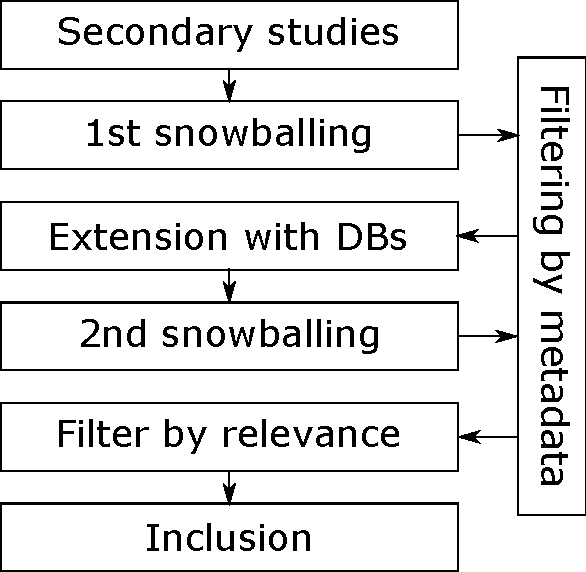
\includegraphics[]{figure/literature_review_process.pdf}
    \caption{Literature review process followed for this study.}
    \label{fig:literature_review_process}
\end{figure}
    


\todo{Fix the Literature reivew process with more details}
\todo{Create table with the numeric results}
